\textbf{Bertrand's Ballot Theorem} \\
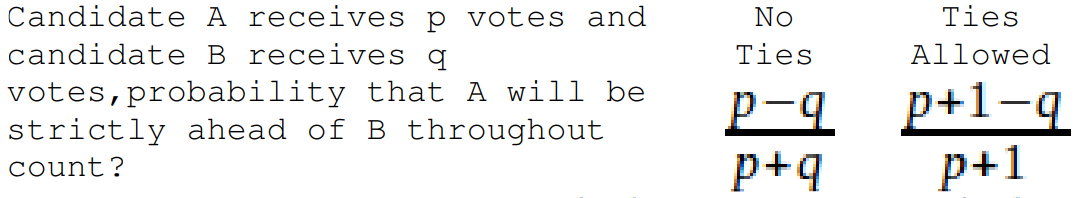
\includegraphics[width=\linewidth]{source/5-maths/Temporary/bertrandBallot.png}

\textbf{Gambler's Ruin Theorem} \\
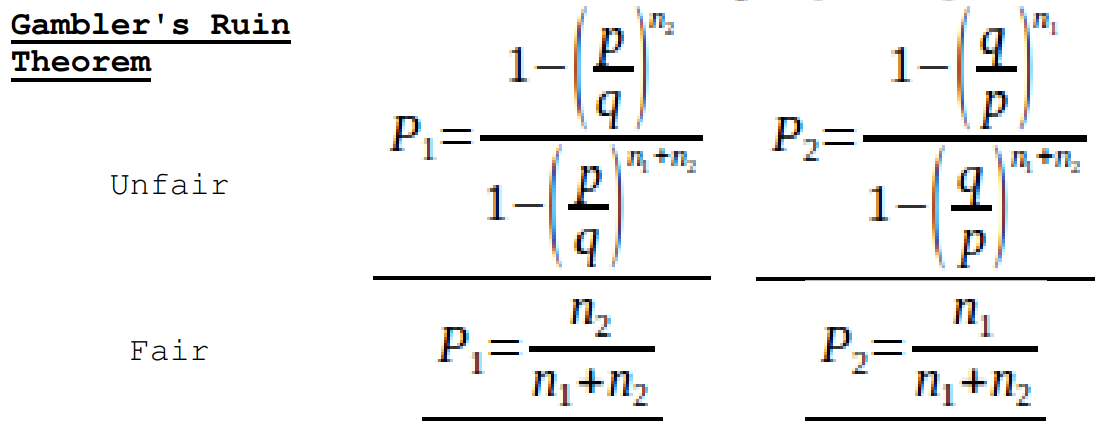
\includegraphics[width=\linewidth]{source/5-maths/Temporary/gamblersRuin.png}

\textbf{Pick Theorem} \\
Let A : the area of a simply closed lattice polygon; B : the number of lattice points on the Polygon edges; I : the number of points in the interior of the polygon. Then \textbf{A = I+(1/2)B-1}

\textbf{Forbenius Number} \\
If GCD is 1 then required largest amount is (X*Y)-(X+Y) and total count is (X-1)*(Y-1)/2

\textbf{Erdos Gallai Theorem} \\
A sequence of non-negative integers $ d_1 \leq \dotsc \leq d_n $, can be represented as the degree sequence of a finite simple graph on n vertices if and only if $ d_1 + \dotsc + d_n $ is even and $ \sum_{i=1}^{i=k} d_i \leq k (k-1) + \sum_{i=k+1}^{i=n} min(d_i,k) $, holds every $ 1 \leq k \leq n $.

\textbf{Derangement}
\begin{lstlisting}[language=c++]
ll der[15];   der[0] = 1;   der[1] = 0;
REP(i,2,10) der[i] = ((ll)i-1)*(der[i-1]+der[i-2]);
\end{lstlisting}

\textbf{Bell Number} \\
The number of ways a set of n elements can be partitioned into nonempty subsets
\begin{lstlisting}[language=c++]
ll bell[25+5][25+5];   bell[0][0] = 1;
REP(i,1,maks){
	bell[i][0] = bell[i-1][i-1];
	REP(j,1,i)bell[i][j]=bell[i-1][j-1]+bell[i][j-1];
} // Example : n=10 ==> bell[10][0]
\end{lstlisting}

\textbf{Stirling Number 2nd Kind} \\
The number of ways a set of n elements into k subsets) \\
Recurrence : S(n,k) = k*S(n-1,k) + S(n-1,k-1)
\begin{lstlisting}[language=c++]
int stir[n+1][k+1];
for (int i=0; i<=n; i++) stir[i][0] = 0;
for (int i=0; i<=k; i++) stir[0][k] = 0;
REP(i,1,n) REP(j,1,i){
	if (j == 1 || i == j) stir[i][j] = 1;
	else stir[i][j] = j*stir[i-1][j] + stir[i-1][j-1];
} // Example : n=3,k=1 : stir[3][1]
\end{lstlisting}

\textbf{Carmichael Number} \\
Composite numbers n such that a\^(n-1) == 1 (mod n) for every a coprime to n.
\begin{lstlisting}[language=c++]
// 561, 1105, 1729, 2465, 2821, 6601, 8911, 10585
// 15841, 29341, 41041, 46657, 52633, 62745, 63973
// 75361, 101101, 115921, 126217, 162401, 172081
// 188461, 252601, 278545, 294409, 314821, 334153
// 340561, 399001, 410041, 449065, 488881, 512461
\end{lstlisting}

\textbf{Vandermonde Convolution} \\
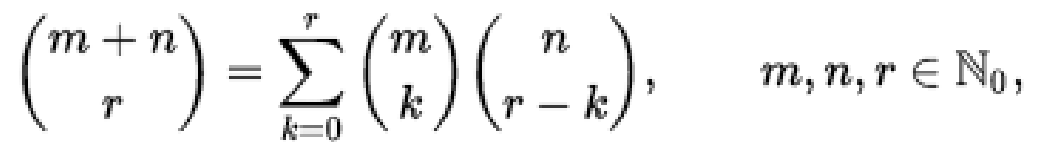
\includegraphics[width=\linewidth]{source/5-maths/Temporary/vandermonde.png}

\textbf{Q-Vandermonde Convolution} \\
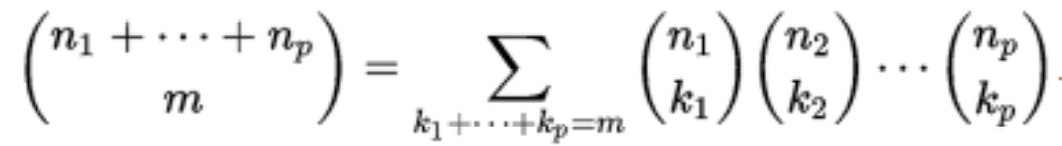
\includegraphics[width=\linewidth]{source/5-maths/Temporary/qVandermonde1.png}
\begin{multicols}{2}
	int m,n \\
	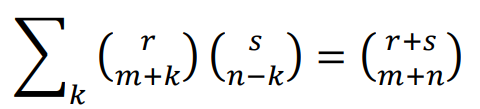
\includegraphics[width=\linewidth]{source/5-maths/Temporary/qVandermonde2.png} \\
	int $l \geq 0$, int m,n \\
	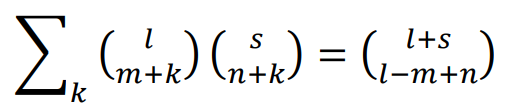
\includegraphics[width=\linewidth]{source/5-maths/Temporary/qVandermonde3.png}
\end{multicols}
int $l \geq 0$, int m,n \\
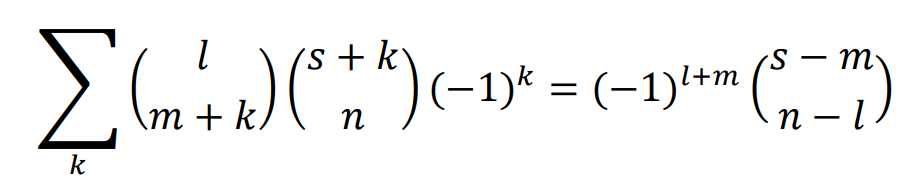
\includegraphics[width=\linewidth]{source/5-maths/Temporary/qVandermonde4.png} \\
int l,m, $m \geq 0$ \\
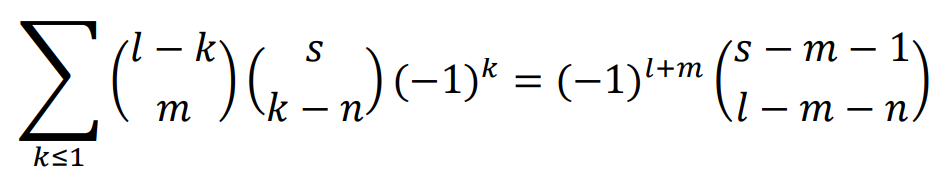
\includegraphics[width=\linewidth]{source/5-maths/Temporary/qVandermonde5.png} \\
int $l,m \geq 0$, int $n \geq q \geq 0$ \\
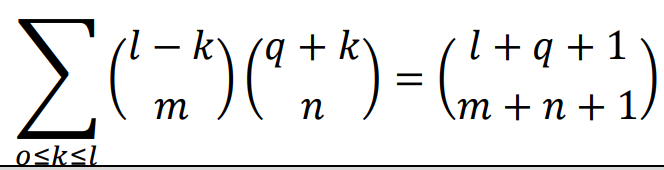
\includegraphics[width=\linewidth]{source/5-maths/Temporary/qVandermonde6.png}
